\section{GUI}

\subsubsection{Klassendiagramm}

\begin{figure}[htbp] 
  \centering
  		 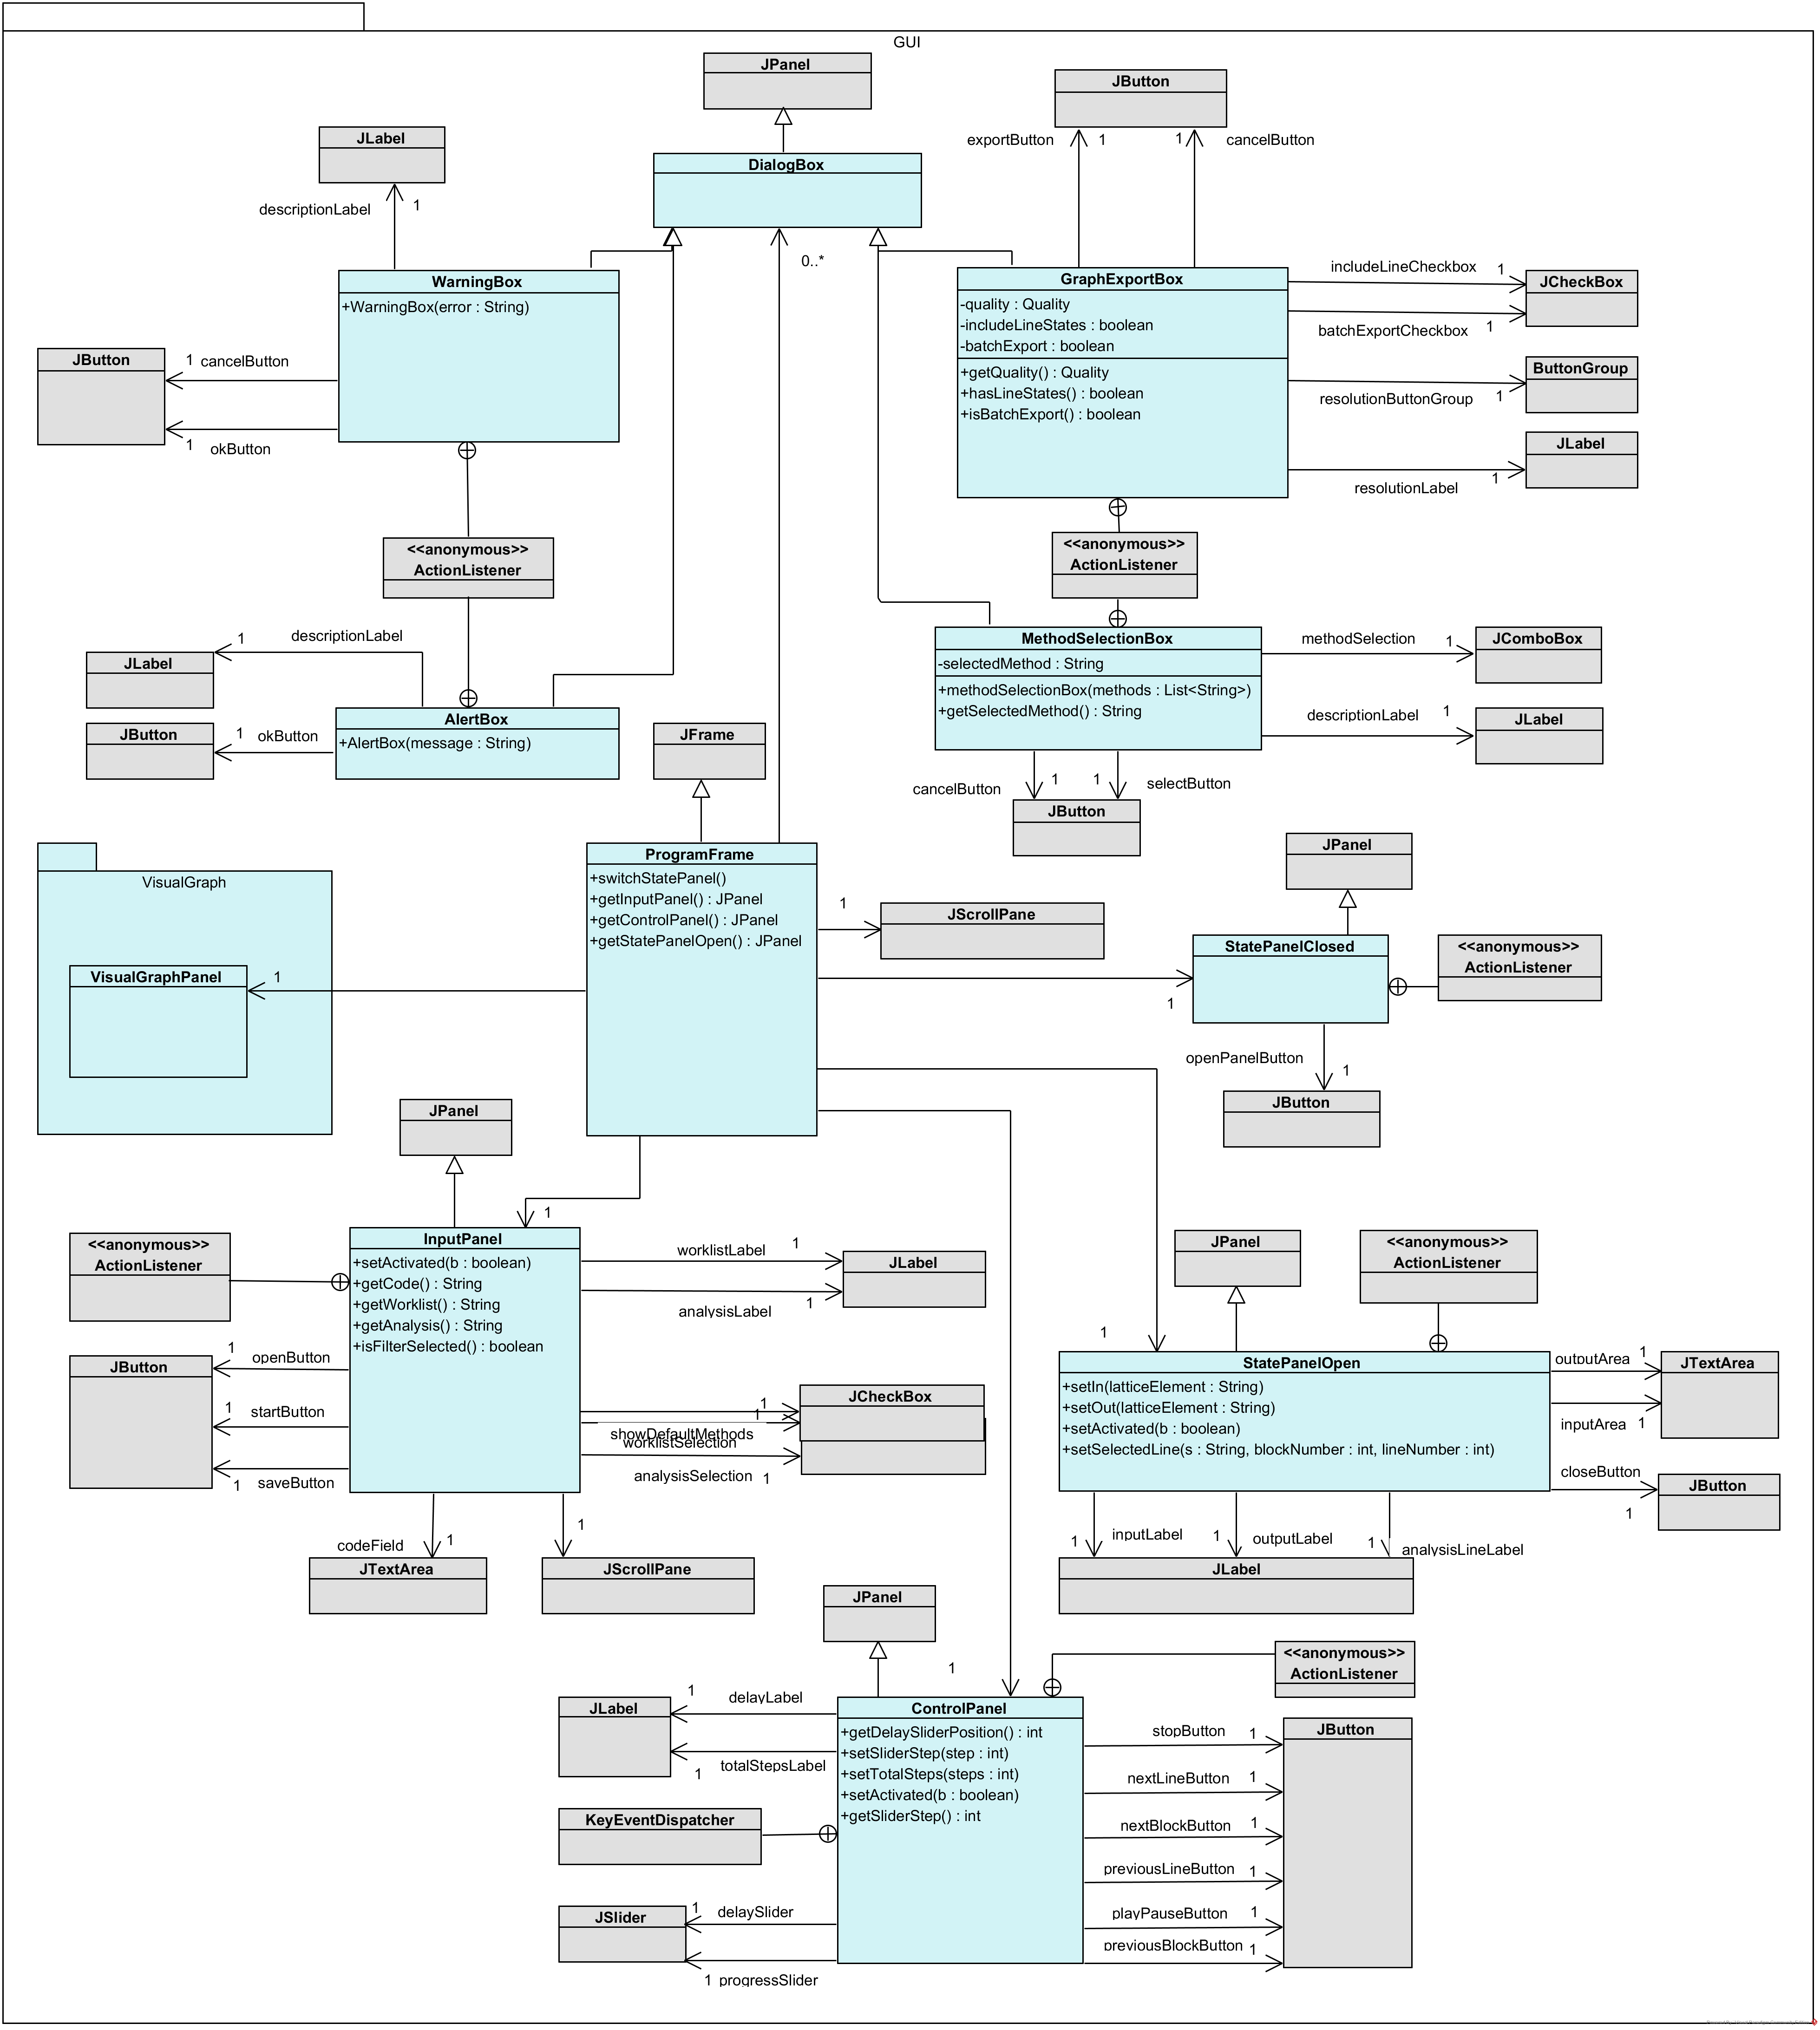
\includegraphics[width=1\textwidth]{Klassenuebersicht/GUI/GUI}
  \caption{Klassendiagramm des User Interfaces}
  \label{fig:UI}
\end{figure}

Das User Interface bildet die zentrale Schnittstelle für die Interaktion mit dem Benutzer.
Es ist aus vier zentralen Panels aufgebaut. 
Das \inlinecode{InputPanel} stellt die für den Benutzer notwendige Funktion für das Einlesen von Code, das Auswählen der Analyse oder des Worklist-Algorithmus und das Starten der Analyse zur Verfügung. 
Nach dem Starten der Analyse kann der Benutzer über das \inlinecode{ControlPanel} die Animation seiner Analyse kontrollieren. 
Die Änderungen, die sich dadurch am Graphen ergeben, werden im \inlinecode{VisualGraphPanel} angezeigt. 
Dieses ist in ein eigenes Modul, welches sich nur um die Visualisierung des Graphen in den verschiedenen Zuständen und um die Interaktion mit dem DFAFramework kümmert, ausgelagert. 
Das \inlinecode{StatePanel} zeigt die In- und Out-States der ausgewählten Zeile oder des ausgewählten Blocks an. 
Des Weiteren wird hier der Aufbau von vier verschiedenen \inlinecode{DialogBoxes} beschrieben. Diese dienen dazu, den Graph zu exportieren, zu analysierende Methoden auszuwählen und den Benutzer zu warnen oder über Fehler zu informieren. 

\subsubsection{Klassenbeschreibung}


\paragraph{ProgramFrame} $\;$ \\
\textbf{extends:} JFrame

\subparagraph{Attribute}
\begin{itemize}
	\item \attr{InputPanel}{JPanel}{private}{
		Panel, welches für die Eingabe des zu analysierenden Codes und für die Auswahl von Analyseart und Worklistalgorithmus verantwortlich ist.
	}
	\item \attr{ControlPanel}{JPanel}{private}{
		Panel, über welches der Benutzer die Animation während der Analyse des Codes steuern kann.
	}
	\item \attr{StatePanelOpen}{JPanel}{private}{
		Panel, in welchem dem Benutzer Informationen über die In- und Out-States des ausgewählten Blocks angezeigt werden.
	}
	\item \attr{StatePanelClosed}{JPanel}{private}{
		Panel, welches dargestellt wird, falls das StatePanel ausgeblendet wurde.
	}
	\item \attr{VisualGraphPanel}{JPanel}{private}{
		Panel, in welchem der Kontrollflussgraph dargestellt wird.
	}
\end{itemize}


\subparagraph{Methoden}
\begin{itemize}
	\item \method{switchStatePanel}{void}{}{public}{
		Macht entweder das StatePanelOpen, in dem die In- und Out-Informationen gegeben werden sichtbar und blendet StatePanelClosed aus oder blendet StatePanelOpen aus und blendet StatePanelClosed ein. 
	}
	\item \method{getInputPanel}{JPanel}{}{public}{
	Gibt das InputPanel zurück.
	}
	\item \method{getControlPanel}{JPanel}{}{public}{
	Gibt das ControlPanel zurück.
	}
	\item \method{getStatePanel}{JPanel}{}{public}{
	Gibt das StatePanelOpen zurück.
	}
\end{itemize}

\paragraph{InputPanel} $\;$ \\
\textbf{extends:} JPanel

\subparagraph{Attribute}
\begin{itemize}
	\item \attr{codeField}{JTextArea}{private}{
		Textfeld, in welchem der zu analysierende Code steht.
	}
	\item \attr{startButton}{JButton}{private}{
		Button, mit welchem der Benutzer die Analyse starten kann.
	}
	\item \attr{openButton}{JButton}{private}{
		Button, mit welchem der Benutzer eine .java-Datei aus seinem Dateisystem öffnen kann.
	}
	\item \attr{saveButton}{JButton}{private}{
		Button, mit welchem der angezeigte Code als .java-Datei gespeichert werden kann.
	}
	\item \attr{worklistLabel}{JLabel}{private}{
		Label, auf welchem steht, dass im Folgenden der Worklistalgorithmus ausgewählt werden kann.
	}
	\item \attr{analysisLabel}{JLabel}{private}{
		Label, auf welchem steht, dass im Folgenden die Analyse ausgewählt werden kann.
	}
	\item \attr{showDefaultMethods}{JCheckBox}{private}{
		Checkbox, durch welche bestimmt wird, ob Standardmethoden in der Methodenauswahl zur Verfügung stehen.
	}
	\item \attr{worklistSelection}{JComboBox}{private}{
		In dieser Auswahl kann der Worklistalgorithmus bestimmt werden.
	}
	\item \attr{analysisSelection}{JComboBox}{private}{
		In dieser Auswahl kann die Analyse ausgewählt werden.
	}
\end{itemize}


\subparagraph{Methoden}
\begin{itemize}
	\item \method{setActivated}{void}{active : boolean}{public}{
		Bestimmt, ob das InputPanel gerade verwendet werden kann oder nicht. Läuft eine aktuelle Analyse, ist das InputPanel deaktiviert und wird erst beim Abbruch der aktuellen Analyse wieder aktiv.
	}
	\item \method{getCode}{String}{}{public}{
		Gibt den aktuell angezeigten Java-Code zurück.
	}
	\item \method{getWorklist}{String}{}{public}{
		Gibt den Namen des aktuell ausgewählten Worklist-Algorithmus zurück.
	}
	\item \method{getAnalysis}{String}{}{public}{
		Gibt den Namen der aktuell ausgewählten Analyse zurück.
	}
	\item \method{isFilterSelected}{boolean}{}{public}{
		Gibt zurück, ob die Methoden gefiltert werden sollen oder nicht.
	}
\end{itemize}


\paragraph{ControlPanel} $\;$ \\
\textbf{extends:} JPanel

\subparagraph{Attribute}
\begin{itemize}
	\item \attr{delaySlider}{JSlider}{private}{
		Slider, mit welchem das Delay beim automatischen Durchlaufen der Analyse bestimmt werden kann.
	}
	\item \attr{progressSlider}{JSlider}{private}{
		Slider, mit welchem der Schritt der Analyse ausgewählt werden kann.
	}
	\item \attr{stopButton}{JButton}{private}{
		Button, mit welchem die Analyse abgebrochen werden kann.
	}
	\item \attr{nextLineButton}{JButton}{private}{
		Button, durch welchen die nächste Zeile im Graphen analysiert und die Darstellung dementsprechend geändert wird.
	}
	\item \attr{nextBlockButton}{JButton}{private}{
		Button, durch welchen der nächste Block im Graphen analysiert und die Darstellung dementsprechend geändert wird.
	}
	\item \attr{previousLineButton}{JButton}{private}{
		Button, durch welchen zum Zustand der Analyse in der vorherigen Zeile zurückgekehrt wird.
	}
	\item \attr{previousBlockButton}{JButton}{private}{
		Button, durch welchen zum Zustand der Analyse im vorherigen Block zurückgekehrt wird.
	}
	\item \attr{playPauseButton}{JButton}{private}{
		Button, mit welchem die automatische Wiedergabe der Analyse gestartet und pausiert werden kann.
	}
	\item \attr{totalStepsLabel}{JLabel}{private}{
		Label, auf welchem die Gesamtanzahl der Schritte der Analyse steht.
	}
	\item \attr{delayLabel}{JLabel}{private}{
		Label, durch welches der DelaySlider beschriftet wird.
	}
\end{itemize}


\subparagraph{Methoden}
\begin{itemize}
	\item \method{getDelaySliderPosition}{int}{}{public}{
		Gibt die Position des DelaySliders zurück.
	}
	\item \method{setSliderStep}{void}{step : int}{public}{
		Setzt die Position des StepSliders an den übergebenen Schritt.
	}
	\item \method{getSliderStep}{int}{}{public}{
		Gibt die Position des StepSliders zurück.
	}
	\item \method{setTotalSteps}{void}{steps: int}{public}{
		Schreibt die Gesamtanzahl der Schritte, die die Analyse macht, in das totalStepsLabel.
	}
	\item \method{setActivated}{void}{active: boolean}{public}{
		Bestimmt, ob das ControlPanel gerade verwendet werden kann oder nicht. Läuft eine aktuelle Analyse, ist das ControlPanel aktiviert und wird erst beim Abbruch der aktuellen Analyse deaktiviert.	
		}
\end{itemize}


\paragraph{StatePanelOpen} $\;$ \\
\textbf{extends:} JPanel

\subparagraph{Attribute}
\begin{itemize}
	\item \attr{analysisLineLabel}{JLabel}{private}{
		Label, auf welchem steht, an welcher Position sich die Analyse befindet.
	}
	\item \attr{inputLabel}{JLabel}{private}{
		Label, durch welches der Beginn der inputArea angezeigt wird.
	}
	\item \attr{outputLabel}{JLabel}{private}{
		Label, durch welches der Beginn der outputArea angezeigt wird.
	}
	\item \attr{inputArea}{JTextArea}{private}{
		Textfeld, in welcher der In-State der aktuell ausgewählten Komponente steht.
	}
	\item \attr{outputArea}{JTextArea}{private}{
		Textfeld, in welcher der out-State der aktuell ausgewählten Komponente steht.
	}
	\item \attr{closeButton}{JButton}{private}{
		Button, mit welchem das StatePanel geschlossen werden kann.
	}
\end{itemize}


\subparagraph{Methoden}
\begin{itemize}
	\item \method{setIn}{void}{latticeElement : String}{public}{
		Zeigt die Text-Repräsentation des übergebenen LatticeElements für in den In-State in dem entsprechenden Textfeld an.
	}
	\item \method{setOut}{void}{latticeElement : String}{public}{
		Zeigt die Text-Repräsentation des übergebenen LatticeElements für in den Out-State in dem entsprechenden Textfeld an.
	}
	\item \method{setSelectedLine}{void}{content : String, blockNumber : int, lineNumber : int}{public}{
		Zeigt die Text-Repräsentation des ausgewählten Blocks oder der ausgewählten Zeile im entsprechenden Textfeld an und fügt die Nummer des Blockes oder der Zeile hinzu.
	}
	\item \method{setActivated}{void}{active : boolean}{public}{
		Bestimmt, ob das StatePanelOpen gerade verwendet werden kann oder nicht. Läuft eine aktuelle Analyse, ist das StatePanelOpen aktiviert und wird erst beim Abbruch der aktuellen Analyse wieder deaktiviert.
	}
\end{itemize}

\paragraph{StatePanelClose} $\;$ \\
\textbf{extends:} JPanel

\subparagraph{Attribute}
\begin{itemize}
	\item \attr{openPanelButton}{JButton}{private}{
		Button, mit welchem das StatePanelOpen geöffnet werden kann.
	}
\end{itemize}



\paragraph{DialogBox} $\;$ \\
\textbf{extends:} JPanel

\subparagraph{Attribute}
\begin{itemize}
	\item \attr{title}{String}{private}{
		Bestimmt den Titel der Dialogbox.
	}
\end{itemize}


\paragraph{MethodSelectionBox} $\;$ \\
\textbf{extends:} DialogBox

\subparagraph{Attribute}
\begin{itemize}
	\item \attr{selectedMethod}{String}{private}{
		String, in welchem die ausgewählte Methode gespeichert wird.
	}
	\item \attr{methodSelection}{JComboBox}{private}{
		ComboBox, in welcher alle Methoden aufgelistet sind und aus ihnen ausgewählt werden kann.
	}
	\item \attr{descriptionLabel}{JLabel}{private}{
		Label, in welchem erklärende Anweisungen gegeben werden.
	}
	\item \attr{cancelButton}{JButton}{private}{
		Button, mit welchem der Vorgang abgebrochen werden kann.
	}
	\item \attr{selectButton}{JButton}{private}{
		Button, mit welchem das Fenster geschlossen und die Methode endgültig ausgewählt werden kann.
	}
\end{itemize}


\subparagraph{Methoden}
\begin{itemize}
	\item \method{methodSelectionBox}{void}{methods : List<String>}{public}{
		Übergibt eine Liste von im Code vorhandenen Methoden, zwischen denen ausgewählt werden können soll.
	}
	\item \method{getSelectedMethod}{String}{}{public}{
		Gibt zurück, welche Methode aktuell ausgewählt ist.
	}
\end{itemize}


\paragraph{GraphExportBox} $\;$ \\
\textbf{extends:} DialogBox

\subparagraph{Attribute}
\begin{itemize}
	\item \attr{quality}{Quality}{private}{
		Legt die ausgewählte Qualität fest.
	}
	\item \attr{includeLineStates}{boolean}{private}{
		Gibt an, ob LineStates in den BatchExport integriert werden sollen.
	}
	\item \attr{batchExport}{boolean}{private}{
		Gibt an, ob BatchExport ausgewählt wurde.
	}
	\item \attr{batchExportCheckBox}{JCheckBox}{private}{
		CheckBox, in der ausgewählt wird, ob ein BatchExport durchgeführt wird.
	}
	\item \attr{includeLineCheckBox}{JCheckBox}{private}{
		CheckBox, in der ausgewählt wird, ob LineStates integriert werden.
	}
	\item \attr{resolutionButtonGroup}{ButtonGroup}{private}{
		Buttons, durch welche die Qualität bestimmt werden kann.
	}
	\item \attr{exportButton}{JButton}{private}{
		Button, mit welchem die Eingaben bestätigt und der Export durchgeführt werden kann.
	}
	\item \attr{cancelButton}{JButton}{private}{
		Button, mit welchem der Vorgang abgebrochen werden kann.
	}
	\item \attr{resolutionLabel}{JLabel}{private}{
		Label, das beschreibt, was im Folgenden gewählt werden kann.
	}
\end{itemize}


\subparagraph{Methoden}
\begin{itemize}
	\item \method{getQuality}{Quality}{}{public}{
		Gibt die ausgewählte Qualität zurück.
	}
	\item \method{hasLineStates}{boolean}{}{public}{
		Gibt zurück, ob die Zeilen in den BatchExport mit aufgenommen werden sollen.
	}
	\item \method{isBatchExport}{boolean}{}{public}{
		Gibt zurück, ob BatchExport ausgewählt wurde.
	}
\end{itemize}


\paragraph{WarningBox} $\;$ \\
\textbf{extends:} JPanel

\subparagraph{Attribute}
\begin{itemize}
	\item \attr{descriptionLabel}{JLabel}{private}{
		Label, in welchem der Fehler ausgegeben wird.
	}
	\item \attr{cancelButton}{JButton}{private}{
		Button, mit welchem der Vorgang abgebrochen werden kann.
	}
	\item \attr{okButton}{JButton}{private}{
		Button, damit der Vorgang trotzdem durchgeführt wird.
	}
\end{itemize}


\subparagraph{Konstruktoren}
\begin{itemize}
	\item \ctor{WarningBox}{message: String}{public}{
		Schreibt die entsprechende Nachricht in das Label.
	}
\end{itemize}


\paragraph{AlertBox} $\;$ \\
\textbf{extends:} DialogBox

\subparagraph{Attribute}
\begin{itemize}
	\item \attr{descriptionLabel}{JLabel}{private}{
		Label, in welchem die Fehlermeldung ausgegeben wird.
	}
	\item \attr{okButton}{JButton}{private}{
		Button, mit welchem sich das Fenster wieder schließt.
	}
\end{itemize}


\subparagraph{Konstruktoren}
\begin{itemize}
	\item \ctor{AlertBox}{error : String}{public}{
		Schreibt die entsprechende Nachricht in das Label.
	}
\end{itemize}